\section{Design of the Protocol}
\label{sec:external-design}

In designing the Externally Secure CC Protocol, we do not add any computationally expensive operations such as signature verification, or even hashing on the credit card:
    beyond its current function, we restrict a credit card to performing only basic arithmetic, indexing, XOR, and similarly inexpensive operations.
We design the protocol using a process called \emph{stepwise refinement}:
\begin{enumerate}
\item First, we define the protocol in terms of an abstract function \emph{H}.
\item We then identify two desired properties of function \emph{H}, namely \textbf{H1} and \textbf{H2},
	and show that if function \emph{H} satisfies these two properties,
	then the protocol is not vulnerable to the four classes of attacks described in Section \ref{sec:insecure-attacks}.
\item Next, we define function \emph{H} in terms of two abstract functions \emph{F} and \emph{G}.
We then identify three properties, namely \textbf{F1}, \textbf{F2}, and \textbf{G1},
	and prove that if function \emph{F} satisfies properties \textbf{F1} and \textbf{F2}
	and function \emph{G} satisfies property \textbf{G1}, then function \emph{H} satisfies the two desired properties \textbf{H1} and \textbf{H2}.
\item We then propose concrete implementations of functions \emph{F} and \emph{G}.
\item Finally, we argue that our proposed implementation of function \emph{F} satisfies properties \textbf{F1} and \textbf{F2},
	and that our proposed implementation of function \emph{G} satisfies property \textbf{G1}.
\end{enumerate}

In so doing, we provide a concrete implementation of the Externally Secure CC Protocol
	and show that it is not vulnerable to any of the four classes of outsider attacks described in Section \ref{sec:insecure-attacks}.

The Externally Secure CC Protocol uses the same four messages that are used in the Insecure CC Protocol.
However, the contents of these messages have become more involved.
In particular, we incorporate a challenge-response mechanism in the Solicitation and Card Information messages.
An outline of this protocol is shown in Figure \ref{fig:external-ccp}.

\begin{figure}[h!]
  \caption{Externally Secure CC Protocol}
  \centering
    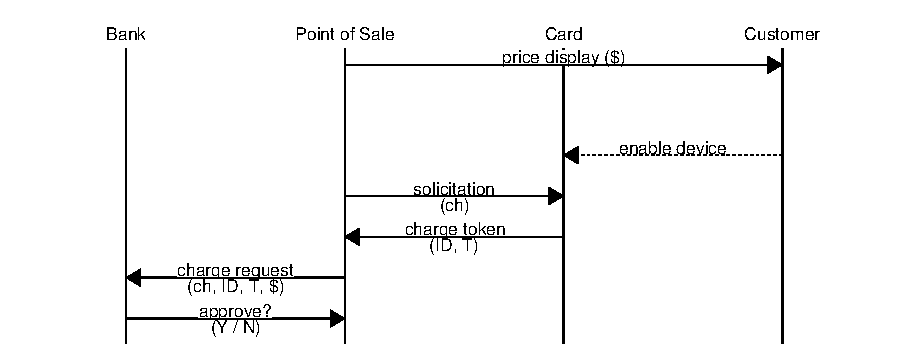
\includegraphics{img/external_ccp.eps}
  \label{fig:external-ccp}
\end{figure}

The four messages used in the Externally Secure CC Protocol are as follows:

\begin{description}
\item[Solicitation (\emph{ch}):]
The point of sale sends a Solicitation message much like in the Insecure CC Protocol.
However, this message now includes a random challenge \emph{ch}.
This challenge is used by the credit card when constructing its response.

\item[Card Information (\emph{ID}, \emph{T}):]
The credit card's response consists of two primary components, ID and T. They are as follows:

\begin{description}
\item[\emph{ID},]a Universally Unique Identifier \cite{uuid}, is used to identify the card without revealing the card's information to eavesdroppers or any other party.
This value is computed by the credit card manufacturer and stored on the card as a constant.

\item[\emph{T = H(info, ch, iCVV)}] is used to authenticate the card's identity.
This abstract function \emph{H} will be defined later through stepwise refinement, but informally we can think of it as similar to a cryptographic hash function:
	it can be used to verify its arguments while leaking no information about them.
\end{description}

In so doing, \emph{ID} provides identification and \emph{T} provides authentication.
In addition, this message is accompanied by the bank name \emph{B}, as before, so that the point of sale may route its Charge Request to the proper entity.

\item[Charge Request (\emph{ID}, \emph{T}, \emph{ch}, \emph{\$}):]
After receiving the Card Information message, the point of sale issues a Charge Request to the credit card's issuing bank.
The point of sale does not learn the card's private information, but simply forwards the card identification (\emph{ID}) and authentication (\emph{T}) to the bank \emph{B},
    specified in the Card Information message.
The point of sale also includes the challenge \emph{ch}
	(so that the bank can verify that \emph{T} is a valid response to \emph{ch} from card \emph{ID}),
	as well as the dollar amount to be charged.

\item[Approval (Y/N):]
The bank maintains an index of \emph{ID} into its account database.
When the bank receives a Charge Request message, it identifies the matching record as specified by \emph{ID}, looking up $\textrm{\emph{info}}_{bank}$ and $iCVV_{bank}$.
It then calculates $T_{bank} = H(\textrm{\emph{info}}_{bank},~ ch,~ iCVV_{bank})$ and verifies that $T = T_{bank}$.
This step is equivalent to verifying the credit card information and iCVV in the Insecure CC Protocol,
	and results in a decision to accept or reject the charge request.

\end{description}





\subsection{Desired Properties of Function \emph{H}}
\label{external-h-properties}

We pit the Externally Secure CC Protocol against the attacks described in Section \ref{sec:insecure-attacks}
	and identify the two properties \textbf{H1} and \textbf{H2} needed from function \emph{H} in order for these attacks to be thwarted.

\subsubsection*{Defending Against Eavesdropping}
When eavesdropping on a transaction, the eavesdropper learns a valid (\emph{ch}, \emph{ID}, \emph{T}, \emph{B}) tuple.
The challenge \emph{ch}, the card identifier \emph{ID}, and the bank name \emph{B} are all public information, of no value to the eavesdropper.
Only $T = H(\textrm{\emph{info}},~ ch,~ iCVV)$ contains authentication information useful to an eavesdropper.
In order to guarantee that no sensitive information is leaked, we require that function \emph{H} satisfies the following property:

\begin{description}
\item[H1:] If \emph{iCVV} is indistinguishable from random, then $H(\textrm{\emph{info}},~ ch,~ iCVV)$ is indistinguishable from random.
\end{description}

If function \emph{H} satisfies property \textbf{H1}, then the eavesdropper (ignorant of \emph{iCVV}) cannot distinguish \emph{T} from random and gains no useful information.








\subsubsection*{Defending Against Skimming}
When sending a Solicitation message to a credit card, the skimmer includes a challenge $ch_{skim}$, which the card uses to construct its response.
From the resulting Card Information message, the skimmer learns \emph{ID}, $T_{skim} = H(\textrm{\emph{info}}, ch_{skim}, iCVV)$ and \emph{B}.
When the skimmer attempts to perform a purchase using this information, it will be issued a challenge $ch_{pos}$ by the point of sale.
In order to prevent the skimmer from correctly responding to this challenge, we require that function \emph{H} satisfies the following property:

\begin{description}
\item[H2:] Given $H(\textrm{\emph{info}},~ ch,~ iCVV)$, \emph{ch}, and $ch'$ such that $ch \neq ch'$, one cannot infer $H(\textrm{\emph{info}},~ ch',~ iCVV)$.
\end{description}

If function \emph{H} satisfies property \textbf{H2}, then the skimmer cannot use the value of $T_{skim}$ in order to construct a response to the point of sale's challenge $ch_{pos}$, and thus cannot perform purchases on behalf of the credit card.






\subsubsection*{Defending Against Relay Attacks}
The relay attack operates similarly to the skimming attack.
When performing a relay attack, the relay provides challenge $ch_{relay}$ to the card.
As in the skimming attack, the relay learns \emph{ID}, $T_{relay} = H(\textrm{\emph{info}},~ ch_{relay},~ iCVV)$, and \emph{B}, and then transmits this information to the proxy.
When the proxy attempts to perform a purchase, it is issued a challenge $ch_{pos}$ by the point of sale.

Thus, if function \emph{H} satisfies the property \textbf{H2},
	then the proxy cannot use the value of $T_{relay}$ in order to construct a valid response to the point of sale's challenge $ch_{pos}$,
	and as a result, cannot perform this purchase on behalf of the credit card.






\subsubsection*{Defending Against Compromised Points of Sale}
A compromised point of sale will result in an attacker learning a valid (\emph{ch}, \emph{ID}, \emph{T}, \emph{B}) tuple,
	which the point of sale requires in order to construct a Charge Request message.
Note that this is the same information learned by the attacker in the eavesdropping case.
As such, if the function \emph{H} satisfies property \textbf{H1}, then the information learned by a compromised point of sale is of no value:
	no private information about the credit card is leaked,
	and the authentication token \emph{T} cannot be reused since the \emph{iCVV} used in its construction is no longer valid after the charge has occurred.



In summary, in order to defend against the four classes of attacks described in Section \ref{sec:insecure-attacks},
	we require that the \emph{iCVV} be a pseudorandom value, and that function \emph{H} upholds the following two properties:

\begin{description}
\item[H1:] If \emph{iCVV} is indistinguishable from random, then $H(\textrm{\emph{info}},~ ch,~ iCVV)$ is indistinguishable from random.
\item[H2:] Given $H(\textrm{\emph{info}},~ ch,~ iCVV)$, \emph{ch}, and $ch'$ such that $ch \neq ch'$, one cannot infer $H(\textrm{\emph{info}},~ ch',~ iCVV)$.
\end{description}









\subsection{Implementing Function \emph{H}}

We find it convenient to define function \emph{H} as a composition of functions \emph{F} and \emph{G} as follows:

$H(\textrm{\emph{info}},~ ch,~ iCVV) = F(x,~ iCVV) \textrm{ where } x = G(\textrm{\emph{info}},~ ch)$

Once defined in these terms, we posit the properties \textbf{H1} and \textbf{H2} in terms of functions \emph{F} and \emph{G}.
We then show that if function \emph{F} satisfies the properties \textbf{F1} and \textbf{F2}, and function \emph{G} satisfies the property \textbf{G1},
then function \emph{H} satisfies the desired properties \textbf{H1} and \textbf{H2}.

\begin{description}
\item[F1:] If $y$ is indistinguishable from random, then $F(x, y)$ is indistinguishable from random.
\item[F2:] Given only $x$, or given only $y$, one cannot infer $F(x, y)$.
\item[G1:] Given $G(u, v)$, $v$, and $v'$ such that $v \neq v'$, one cannot infer $G(u, v')$ without knowledge of $u$.
\end{description}

\newtheorem{theorem}{Theorem}

\begin{theorem}
If function \emph{F} satisfies property \textbf{F1}, then function \emph{H} satisfies property \textbf{H1}.
\end{theorem}

\begin{proof}
  Let $x = G(\textrm{\emph{info}},~ ch)$ for any $\textrm{\emph{info}}$,~ $ch$.
  Then $H(\textrm{\emph{info}},~ ch,~ iCVV) = F(x,~ iCVV)$.
  Thus if $y = iCVV$ is indistinguishable from random, then by property \textbf{F1}, $F(x,y) = H(\textrm{\emph{info}},~ ch,~ iCVV)$ is indistinguishable from random.
\end{proof}


\begin{theorem}
If function \emph{F} satisfies property \textbf{F2}, and function \emph{G} satisfies property \textbf{G1}, then function \emph{H} satisfies property \textbf{H2}.
\end{theorem}

\begin{proof}
  Let $x = G(\textrm{\emph{info}},~ ch)$ and $x' = G(\textrm{\emph{info}},~ ch')$ for any $\textrm{\emph{info}}$.
  By property \textbf{F2}, evaluating $H(\textrm{\emph{info}},~ ch',~ iCVV)$ requires knowledge of $x' = G(\textrm{\emph{info}},~ ch')$.
  However, by property \textbf{G1}, one cannot infer $G(\textrm{\emph{info}},~ ch')$ without knowledge of $\textrm{\emph{info}}$.
  Further, by property \textbf{H1}, no bits of $\textrm{\emph{info}}$ are leaked and thus $\textrm{\emph{info}}$ remains secret.
  Thus, given $H(\textrm{\emph{info}},~ ch,~ iCVV)$, $ch$, and $ch'$ such that $ch \neq ch'$, one cannot infer $H(\textrm{\emph{info}},~ ch',~ iCVV)$.
\end{proof}

While $\textrm{\emph{info}}$ is considered secret, it cannot be used directly in function \emph{G}.
This is because while most of the data in $\textrm{\emph{info}}$ is unpredictable, many of the bits are not random.
For example, in a typical credit card number, the first six digits are taken from the \emph{Issuer Identification Number}, a public value assigned to the issuing bank.
Similarly, the attacker can guess the bytes representing the expiration month and year from a very small set of possibilities.
Furthermore, the credit card number and expiration date are transmitted as decimal values transliterated into hexadecimal (e.g. ``4491'' is transmitted as two bytes: \texttt{0x44} and \texttt{0x91}).
As such, inferences may be made about the value of particular bits, since each such byte is drawn from only 154 possible values.

To resolve this problem, we use a keyed hash function known as an HMAC \cite{krawczyk1997hmac} to compute $h_k(\textrm{\emph{info}})$, using a key \emph{k} known only to the bank.
As \emph{info} does not change over the lifetime of the credit card, $h_k(\textrm{\emph{info}})$ is stored as a constant on the card.
As such, the computation necessary for hashing is not executed on the credit card, and the card requires no knowledge of the bank's secret key \emph{k}.
For convenience we will refer to the output of $h_k(\textrm{\emph{info}})$ as the constant \emph{khi}.

We propose implementations for functions \emph{G} and \emph{F} (and thus \emph{H}) in Figure \ref{fig:implementation}.
Note that function \emph{G} is defined as the function which returns those bits of a keyed HMAC $h_k(\textrm{\emph{info}})$ for which the corresponding bit of $ch$ was set to 1.
Also note that function \emph{F} is defined as \texttt{XOR}.

\begin{figure}[h!]
  \caption{Implementation of \emph{F}, \emph{G} and \emph{H}}
  \begin{verbatim}

function G(info, ch):
    const khi = HMAC(bank_key, info)
    result = empty list of bits
    for each of the n bits of ch:
        if the n'th bit of ch is 1:
            append n'th bit of khi to result
    return result

function F(x, iCVV):
    return x XOR iCVV

function H(info, ch, iCVV):
    x = G(info, ch)
    return F(x, iCVV)
\end{verbatim}
  \label{fig:implementation}
\end{figure}

In the Insecure CC Protocol, $\textrm{\emph{info}}$ is composed of 96 bits, and $iCVV$ is composed of 32 bits.
If we maintain these field-lengths in the Externally Secure CC Protocol, and use an HMAC function which also outputs 96 bits, then our implementation of \emph{F} and \emph{G} requires that $ch$ must be a 96 bit value with 32 1's and 64 0's.
More generally, our implementation requires that $h_k(\textrm{\emph{info}})$ and $ch$ have the same number of bits,
	and that the number of \emph{1-bits} in \emph{ch} is equal to the number of bits in \emph{iCVV}.

Note that the \texttt{XOR} operation satisfies properties \textbf{F1} and \textbf{F2}, so our implementation of function \emph{F} (trivially) satisfies them as well.

The output of $G(\textrm{\emph{info}},~ ch)$ is composed of a number of bits of \linebreak $\textrm{\emph{khi}} = h_k(\textrm{\emph{info}})$ selected by the challenge $ch$.
If $ch_1 \neq ch_2$, one cannot infer $G(khi,~ ch_2)$ from $G(khi,~ ch_1)$ without knowledge of $khi$,
because the results are composed of different bits of $khi$ selected by the challenges $ch_1$ and $ch_2$.
These bits are indistinguishable from random to any party without knowledge of $\textrm{\emph{info}}$ and the bank's secret key $k$.
These bits are then masked by the $iCVV$ and as such are not learned by any party.
As a result, our implementation of function \emph{G} satisfies the property \textbf{G1}.
